
\section{Introduction}
\label{sec:introduction}
Modular forms have been for a while a central object in number theory. They have connections to many research areas: arithmetic, combinatorics, analysis, geometry, representation theory,\ldots Since they appear essentially everywhere you look at, it is quite reasonable to wish to understand them.

Here is a not too serious reason: have you ever tried to calculate $e^{\pi\sqrt{163}}$? It turns out that it is
\[
e^{\pi\sqrt{163}} = 262537412640768743.999999999999250072597\ldots
\]
which seems \emph{too close} to an integer to be a coincidence. That is, until you learn about modular forms: it turns out that this number is related to a value of a modular funtion (the $j$-function), which is known to be an integer.

In this introduction I give two more examples that hopefully convince the reader of the importance of modular forms in number theory. You can find many more examples in Zagier's chapter of~\cite{book123modforms}.

\subsection{Partitions and Ramanujan's \texorpdfstring{$\tau$}{tau}-function}
For each $n\geq 0$, define the \emphh{partition function} $p(n)$ as
\[
p(n)=\#\{\text{ways of representing $n$ as a sum of natural numbers }\}.
\]
As a convention, $p(0)=1$. Also, note that:
\begin{align*}
p(1) &= 1\\
p(2) &= 2 = \#\{1+1,2\}\\
p(3) &= 3 = \#\{1+1+1, 1+2, 3\}\\
p(4) &= 5 = \#\{1+1+1+1,1+1+2,1+3,2+2,4\}\\
p(5) &= 7 = \#\{1+1+1+1+1,1+1+1+2,1+1+3,1+4,1+2+2,2+3,5\}\\
\ldots&
\end{align*}
In order to package all these numbers we may consider the following formal powers series:
\[
P(q) = \sum_{n=0}^\infty p(n)q^n,
\]
where we think of $q$ as a formal variable.
\begin{lemma}
  There is an infinite product decomposition
\[
P(q) = \prod_{m=1}^\infty \frac{1}{1-q^m}.
\]
\end{lemma}
\begin{proof}
  We need to look at the right-hand side. Each of the factors can be written as
$\sum_{k=0}^\infty q^{km}$, so the right-hand side looks like
\[
\prod_{m=1}^\infty\sum_{k=0}^\infty q^{km}.
\]
Now we collect the terms contributing to $q^n$, for a fixed $n$. These come from taking $1$ from all but finitely many of the infinite sums, and then collecting $q^{k_1m_1}$, $q^{k_2m_2}$, \ldots, $q^{k_rm_r}$ from $r$ other factors. This is subject to the condition
\[
k_1m_1+k_2m_2+\cdots+k_rm_r = n,
\]
and note that the $m_i$ are all different because they are taken from different factors. There are exactly $p(n)$ such choices, as we wanted to show.
\end{proof}

In view of the previous lemma, a convenient way to study the partition function is through another
very popular function, defined by the following infinite product:
\[
\Delta(q) = q\prod_{n=1}^\infty (1-q^n)^{24}.
\]
Note that we have:
\[
\Delta(q) = q\prod_{n=1}^\infty (1-q^n)^{24} = \frac{q\prod(1-q^n)^{25}}{\prod 1-q^n} = \left(\prod_{n=1}^\infty(1-q^n)^{25}\right) \sum_{n=0}^\infty p(n)q^{n+1}.
\]
We define \emphh{Ramanujan's tau} function via:
\[
\Delta(q)=\sum_{n=1}^{\infty} \tau(n)q^n.
\]

Later in this course you will be able to prove the following striking result.
\begin{theorem}[Ramanujan]
For each $n\geq 1$, we have:
\[
\tau(n)\equiv \sum_{d\mid n} d^{11}\pmod{691}.
\]
Moreover, the partition function satisfies the following congruences:
\[
p(5n+4) \equiv 0\pmod{5},\quad \forall n,
\]
\[
p(7n+5) \equiv 0\pmod{7},\quad \forall n,
\]
\[
p(11n+6) \equiv 0\pmod{11},\quad \forall n.
\]

\end{theorem}
\subsection{A modular form of level \texorpdfstring{$11$}{11} that knows about congruences}
  Consider another modular form:
\[
f(z)=q\prod_{n=1}^\infty (1-q^n)^2(1-q^{11n})^2 = q-2q^2-q^3+2q^4+q^5+2q^6+\cdots = \sum_{n=1}^\infty a(n)q^n.
\]
\begin{theorem}
  \begin{enumerate}
  \item $a(nm) = a(n)a(m)$ whenever $(n,m)=1$.
  \item $|a(p)|\leq 2\sqrt{p}$ for all prime $p$.
  \end{enumerate}
\end{theorem}
Consider the equation:
\[
E\colon Y^2+Y=X^3-X^2-10X-20,
\]
and let $N(p)$ be the number of solutions in $\FF_p$. Heuristically we should think that $N(p)\simeq p$.
\begin{theorem}[Hasse]
  $|p-N(p)|\leq 2\sqrt{p}$.
\end{theorem}

The theory of modular forms allows to prove that the $E$ and $f$ ``correspond'' to each other:
\begin{theorem}
For all primes $p$, we have $a(p) = p - N(p)$.
\end{theorem}
This allows us to easily calculate (from $f$) what is $N(p)$ for all $p$. We say in this case that $E$ ``is modular''. The book~\cite{diamond-shurman} (but not this course) explains how to attach an elliptic curve to a modular form (this is called ``Eichler--Shimura''). It is \textbf{much} harder to reverse this process, and this is what A.~Wiles did in order to prove Fermat's Last Theorem.

\section{The upper half-plane}
\label{sec:upper-half-plane}
This section introduces the seemingly innocuous upper half-plane $\HH$.
\begin{definition}
  The \emphh{upper half-plane} $\HH$ is the set of complex numbers with positive imaginary part:
\[
\HH = \{ z=x+iy ~|~ \Im(z)>0\}.
\]
\end{definition}
The upper half-plane appears in the classification of Riemann surfaces: there are only three of them which are simply connected which are the complex plane, the complex sphere, and $\HH$.

The \emphh{general linear group} $\GL_2(\RR)$ consists of all $2\times 2$ invertible matrices with entries in $\RR$. It contains the subgroup $\GL_2^+(\RR)$ of matrices with positive determinant. The \emphh{special linear group} $\SL_2(\RR)\subset \GL_2^+(\RR)$ consists of those matrices with determinant $1$. For $\gamma=\smtx abcd\in \GL_2(\RR)$ and $z\in\HH$, define $\gamma z$ as:
\begin{equation}
  \label{eq:fractional-linear-transformation}
\gamma z = \mtx abcd z = \frac{az+b}{cz+d}.
\end{equation}
\begin{lemma}
  Let $\gamma=\smtx abcd\in\GL_2(\RR)$. Then:
\[
\Im(\gamma\tau) = \frac{\det(\gamma)}{|c\tau+d|^2}\Im(\tau),\quad \gamma=\mtx abcd.
\]
\end{lemma}

\begin{proof}
  One just needs to compute
\begin{align*}
\Im(\gamma\tau) &= \Im(\frac{a\tau + b}{c\tau+d}) = \Im\left(\frac{(a\tau+b)(c\bar\tau + d)}{|c\tau+d|^2}\right)\\
&= \frac{\Im(ac|\tau|^2 +ad\tau + bc\bar\tau +bd)}{|c\tau+d|^2}=\frac{ad\Im(\tau) - bc\Im(\tau)}{|c\tau+d|^2}.
\end{align*}

\end{proof}
\begin{corollary}
  $\GL_2^+(\RR)$ acts on the left on $\HH$.
\end{corollary}
Note that the determinant gives a decomposition
\[
\GL_2^+(\RR) = \SL_2(\RR) \times \RR,
\]
and since the scalar matrices (those of the form $\smtx{\lambda}{0}{0}{\lambda}$) act trivially on $\HH$, from now on we will restrict our attention to $\SL_2(\RR)$. In fact, since the scalar matrix $\smtx{-1}{0}{0}{-1}$ belongs to $\SL_2(\RR)$, the above action on $\HH$ factors through $\PSL_2(\RR)=\SL_2(\RR)/\{\pm 1\}$, which is called the \emphh{projective special linear group}.

From this action we can deduce a right action on functions on $\HH$, by precomposing:
\[
(f\cdot \gamma)(z) = f(\gamma z).
\]
However, we will need slightly more general actions on functions, but before we introduce a piece of notation that will later prove  useful.

\begin{definition}
  The \emphh{automorphy factor} is the function
\[
j\colon \GL_2^+(\RR)\times \HH \to \CC
\]
given by:
\[
j(\gamma,z) = cz+d,\quad \gamma = \mtx abcd.
\]
\end{definition}
The following lemma gives a very interesting property of the automorphy factor.
\begin{lemma}[cocycle relation]
For every $\gamma_1$, $\gamma_2$ in $\GL_2^+(\RR)$ and for every $z\in\HH$ we have:
\[
j(\gamma_1\gamma_2,z) = j(\gamma_1,\gamma_2z)j(\gamma_2,z).
\]
\end{lemma}
Finally, we define an action of $\GL_2^+(\RR)$ on functions $f\colon\HH\to\CC$, for each $k\in\ZZ$.
\begin{definition}
  The \emphh{weight-$k$ slash operator} is defined as
\begin{equation}
(f|_k\gamma)(z) = (\det \gamma)^{k-1} j(\gamma,z)^{-k}f(\gamma z).
\end{equation}
\end{definition}

The cocycle property and the multiplicativity of the determinant implies that if $f$ is a function, then:
\[
f|_k(\gamma_1\gamma_2) = (f|_k\gamma_1)|_k\gamma_2, \quad \forall \gamma_1,\gamma_2\in\GL_2^+(\RR).
\]
That is, for each $k$ the weight-$k$ slash operator defines an action of $\GL_2^+(\RR)$ on functions on the upper-half plane.

\subsection{Group-theoretic description of \texorpdfstring{$\HH$}{HH}}
Recall that $\SL_2(\RR)$ acts on $\HH$. If $\tau=x+iy\in\HH$, then define
\[
s_\tau =\mtx{y^{1/2}}{xy^{-1/2}}{0}{y^{-1/2}}.
\]
Note that $s_\tau i = \tau$, and therefore $\SL_2(\RR)$ acts transitively on $\HH$.
\begin{lemma}
  The stabilizer in $\SL_2(\RR)$ of $i$ is the compact subgroup of $\SL_2(\RR)$:
\[
\SO_2(\RR)=\left\{\mtx{\cos\theta}{-\sin\theta}{\sin\theta}{\cos\theta} ~|~ \theta\in [0,2\pi]\right\}
\]
\end{lemma}
\begin{proof}
Let $g=\smtx abcd \in\SL_2(\RR)$ stabilize $i$. That means that:
\[
\frac{ai + b}{ci +d} = i,
\]
or equivalently that
\[
ai+b = -c+di.
\]
Since the entries of $g$ are real, this means that $a=d$ and $b=-c$. Therefore $g=\smtx{a}{b}{-b}{a}$. Since moreover $\det(g)=a^2+b^2=1$, we deduce that $g\in \SO_2(\RR)$.
\end{proof}
The lemma gives a bijection:
\[
\HH\to \SL_2(\RR)/\SO_2(\RR),\quad \tau\mapsto s_\tau\SO_2(\RR),
\]
whose inverse maps $g\SO_2(\RR)\mapsto g\cdot i$.

\subsection{The quotient \texorpdfstring{$\SL_2(\ZZ)\backslash \HH$}{SL2\H} as a topological space}
We end this section by showing that the quotient $\SL_2(\ZZ)\backslash \HH$ is a Hausdorff space.
\begin{lemma}
  Let $U_1$ and $U_2$ be two open sets in $\HH$. Then the set
\[
S = \{\gamma\in \SL_2(\ZZ) ~|~ \gamma U_1 \cap U_2 \neq \emptyset\}
\]
is finite.
\end{lemma}
\begin{proof}
  First observe that the matrices $s_{\gamma\tau}$ and $\gamma s_\tau$ both send $i$ to $\gamma\tau$. By the identification $\HH = \SL_2(\RR)/\SO_2(\RR)$ we deduce that $\gamma s_\tau\SO_2(\RR)=s_{\gamma\tau}\SO_2(\RR)$. Given two points $\tau_1$ and $\tau_2$ of $\HH$, we have $\gamma\tau_1 =\tau_2$ if and only if $s_{\gamma\tau_1}\SO_2(\RR) = s_{\tau_2}\SO_2(\RR)$. We have just seen that the left hand side equals $\gamma s_{\tau_1}\SO_2(\RR)$. We deduce that $\gamma\tau_1=\tau_2$ if and only if $\gamma$ belongs to the conjugate: $s_{\tau_2}\SO_2(\RR) s_{\tau_1}^{-1}$. Therefore the set $S$ is a subset of the set
\[
\{\gamma\in\SL_2(\ZZ) ~|~ \gamma \ol U_1 \cap \ol U_2 \neq \emptyset\}
\]
which in turn can be written as
\[
\SL_2(\ZZ)\cap s_{\ol U_2} \SO_2(\RR) s_{\ol U_1}^{-1}.
\]
Since $\SL_2(\ZZ)$ is discrete and the other term is compact, the intersection, and hence $S$, is finite.
\end{proof}
\begin{proposition}
  The action of $\SL_2(\ZZ)$ on $\HH$ is proper discontinuous. That is, given any $\tau_1$, $\tau_2$ in $\HH$, there are neighborhoods $U_1$ and $U_2$ such that for each $\gamma\in \SL_2(\ZZ)$ either
  \begin{enumerate}
  \item $\gamma\tau_1=\tau_2$, or
  \item $\gamma U_1\cap U_2 = \emptyset$.
  \end{enumerate}
\end{proposition}
\begin{proof}
  Let $U_1$ and $U_2$ be any two neighborhoods of $\tau_1$ and $\tau_2$, and let $\gamma\in S$. If $\gamma\tau_1=\tau_2$ then we do not need to do anything. Otherwise, if $\gamma U_1\cap U_2\neq \emptyset$ then we may replace $U_2$ with $V_2$ and $U_1$ with $\gamma^{-1} V_1$ if $V_1\cap V_2=\emptyset$, $\tau_2\in V_2$ and $\gamma\tau_1\in V_1$:
  \begin{figure}[h]
    \centering
    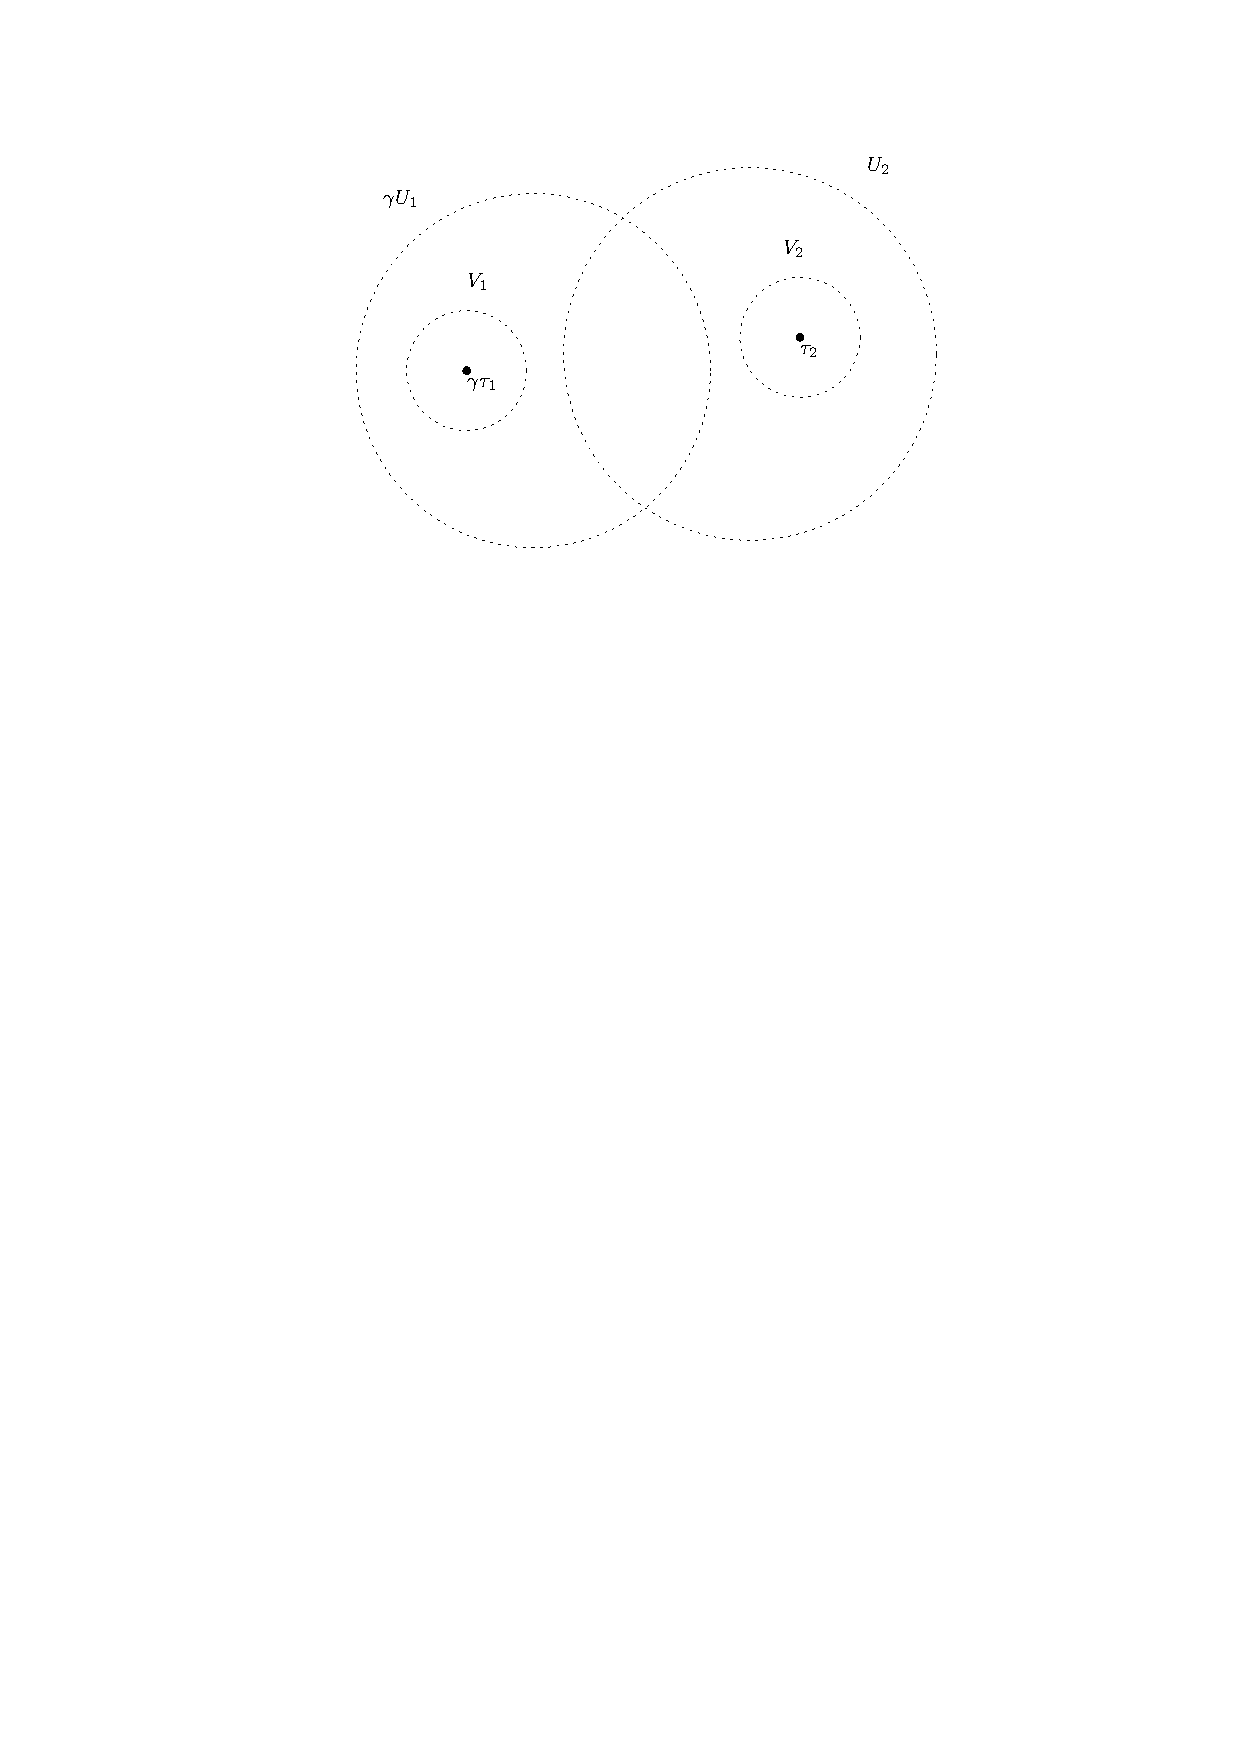
\includegraphics[height=3cm]{Pictures/shrinking-neighborhoods.pdf}
    \caption{Shrinking the neighborhoods}
    \label{fig:shriking-neighborhoods}
  \end{figure}
Since the set of $\gamma$ such that these intersections are nonempty is finite, this process terminates after a finite number of steps and will leave us with the right neighborhoods.
\end{proof}
\begin{corollary}
  The quotient $Y(1) = \SL_2(\ZZ)\backslash\HH$ is Hausdorff.
\end{corollary}
\begin{proof}
  Pick $\pi(\tau_1)\neq \pi(\tau_2)$ in $Y(1)$, and let $U_1$ and $U_2$ be neighborhoods as in the Proposition. For every $\gamma\in\SL_2(\ZZ)$ we have $\gamma\tau_1\neq \tau_2$ by the choice of $\tau_1$ and $\tau_2$. Therefore for every $\gamma\in\SL_2(\ZZ)$ we have $\gamma U_1\cap U_2=\emptyset$. Therefore $\pi(U_1)\cap\pi(U_2)=\emptyset$. It remains to show that $\pi(U_i)$ is an open set. Indeed, if $U\subseteq\HH$ is an open set, then
\[
\pi^{-1}(\pi(U)) = \cup_{\gamma\in\SL_2(\ZZ)} \gamma U
\]
is a union of open sets. Therefore it is open. We have showed that $\pi(U)$ is open (because of the quotient topology). Therefore each of the $\pi(U_i)$ is open, as we wanted to show.
\end{proof}

\section{Basic definitions of modular forms}
\label{sec:the-modular-group}

Let $\SL_2(\ZZ)\subset\SL_2(\RR)$ be the subgroup of matrices with entries in $\ZZ$ (and determinant $1$), which of course still acts on functions as we have seen.
\begin{definition}
  A holomorphic function $f\colon \HH\to\CC$ is called \emphh{weakly-modular} of weight $k\in\ZZ$ for $\SL_2(\ZZ)$ if $f|_k\gamma = f$ for all $\gamma\in\SL_2(\ZZ)$. Explicitly:
\begin{equation}
\label{eq:modular-transformation}
f(\gamma\cdot z) = j(\gamma,z)^k f(z),\quad\forall \gamma\in\SL_2(\ZZ).
\end{equation}

\end{definition}

Note that since $-I\in\SL_2(\ZZ)$, then there are no non-zero weakly-modular functions of odd weight:
\[
f(z)=(-1)^kf(z)\implies f=0.
\]

We will need an extra analytic property to define modular forms for $\SL_2(\ZZ)$. For now, note that:
\[
\frac{d(\gamma\cdot z)}{dz} = j(\gamma,z)^{-2},
\]
so we can rewrite the weakly-modular property by asking that the differential $f(z)(dz)^{k/2}$ is invariant under $\SL_2(\ZZ)$. It also shows that if~\eqref{eq:modular-transformation} holds for $\gamma_1$ and $\gamma_2$, then it also holds for $\gamma_1\gamma_2$.

We will see later (see Corollary~\ref{cor:STgenerate}) that $\SL_2(\ZZ)$ is generated by the matrices $T=\smtx 1101$ and $S=\smtx{0}{-1}{1}{0}$. Together with the previous observation, this implies that for $f$ to be weakly-modular it is enough to check~\eqref{eq:modular-transformation} for $T$ and $S$:
\[
f(z+1)=f(z),\quad f(-1/z) = z^k f(z).
\]

The transformation property (rather, the fact that $f(z+1)=f(z)$) implies that $f$ has a Fourier expansion. Another way to think about it is that there is a holomorphic map:
\[
\exp\colon \HH\to \{0<|q|<1\},\quad z\mapsto q=e^{2\pi i z}.
\]
If $f$ is holomorphic and $1$-periodic, then we can define $g(q)=f(z)$. That is, we may define:
\[
g(q)=f\left(\frac{\log q}{2\pi i}\right),
\]
where we may choose any branch of the logarithm because of the periodicity of $f$. The function $g$ is holomorphic on $D'$, and thus it has a Laurent expansion
\[
g(q)=\sum_{n=-\infty}^\infty a(n)q^n.
\]
Therefore $f$ has an expansion
\[
f(z) = \sum_{n=-\infty}^\infty a(n)e^{2\pi i nz}.
\]
\begin{definition}
  We say that $f$ is \emphh{meromorphic at infinity} (respectively \emphh{holomorphic at infinity}) if $f(z)=\sum_{n\geq n_0} a(n)q^n$ (respectively if in addition $n_0=0$).
\end{definition}
Note that checking that $f$ is holomorphic at infinity is the same as checking that $f(z)$ is bounded as $z$ approaches $i\infty$. If $f$ is holomorphic at infinity, then the value of $f$ at infinity is defined to be $f(\infty)=a(0)$.

\begin{definition}
  We say that $f$ \emphh{vanishes at infinity} if $n_0=1$. Equivalently, if $f(\infty)=0$.
\end{definition}

\begin{definition}
  Let $k\in \ZZ$ and let $f\colon\HH\to\CC$. We say that $f$ is a \emphh{modular form} of weight $k$ for $\SL_2(\ZZ)$ if:
  \begin{enumerate}
  \item $f$ is holomorphic,
  \item $f(\gamma z) = (cz+d)^kf(z)$ for all $\gamma=\smtx abcd\in\SL_2(\ZZ)$, and
  \item $f$ is holomorphic at infinity.
  \end{enumerate}
A \emphh{cusp form} is a modular form which vanishes at infinity.

The space of modular forms of weight $k$ is written $M_k=M_k(\SL_2(\ZZ))$, and it contains the space of cusp forms of weight $k$, which in turn is written $S_k=S_k(\SL_2(\ZZ))$.
\end{definition}


\begin{remark}
  If we replace ``holomorphic'' with ``meromorphic'' above, we obtain
  what can be called \emphh{meromorphic modular forms}. Other authors
  call them modular functions, but this name is used in different
  contexts and we will avoid it.
\end{remark}

Note that both  $M_k$ and $S_k$ are $\CC$-vector spaces. Also, multiplication of functions gives $M=\bigoplus_{k\in\ZZ} M_k$ the structure of a \emph{graded ring}. That is, $M_rM_s\subseteq M_{r+s}$. Finally,
for all odd $k$ one has $M_k = \{0\}$.


\section{Eisenstein series}
\label{sec:fourier-expansions-eisenstein}

For $k\geq 3$, define
\[
G_k(z) = \sumprime_{(m,n)\in \ZZ^2} (mz+n)^{-k}.
\]
\begin{lemma}
  $G_k$ converges absolutely for all $z$, and uniformly on sets of the form
\[
\Omega=\{z\in\HH~|~|\Re(z)|\leq A,\Im(z)\geq B\}.
\]
\end{lemma}
\begin{proof}[Sketch of proof]

First, show that
there exists a constant $C>0$ such that $|z+\delta|>C\sup\{1,|\delta|\}$ for all $z\in\Omega$ and $\delta\in\RR$.

Now, note that:
\begin{align*}
\sumprime |mz+n|^{-k} &= \sumprime |m|^{-k}|z+n/m|^{-k}<\sumprime C^{-k}|m|^{-k}\sup\{1,|n/m|\}^{-k}\\
&=C^{-k}\sumprime \sup\{|m|,|n|\}^{-k}.
\end{align*}
This last sum is easily seen to converge. For instance, one can sum over squares around the origin, of increasing size and compare to a $p$-series.

\end{proof}

The previous lemma ensures that $G_k(z)$ is a holomorphic function. Moreover, we have:
\begin{theorem}
  For each $k\geq 3$, $G_k$ is a modular form.
\end{theorem}

We will first show that $G_k$ is weakly modular.
\begin{proposition}
  For each $k\geq 3$ the holomorphic function $G_k$ is weakly modular.
\end{proposition}
\begin{proof}
Let $\gamma = \smtx abcd$ be a matrix in $\SL_2(\ZZ)$. We compute
\begin{align*}
G_k(\gamma z) &= \sumprime_{(m,n)} \left(m\frac{az+b}{cz+d} + n\right)^{-k}\\
&= \sumprime_{(m,n)} (cz+d)^k \left(m(az+b)+n(cz+d)\right)^{-k}\\
&= (cz+d)^k\sumprime_{(m,n)}\left( (am+cn)z + (bm+dn)\right)^{-k}.
\end{align*}
Note that the pair $(am+cn,bm+dn)$ is the result of multiplying the row vector $(m,n)$ by the matrix $\smtx abcd$. Since $\smtx abcd$ is invertible, the pair $(am+cn,bm+dn)$ runs through all values of $\ZZ^2$ as $(m,n)$ does. Therefore, by reordering the sum above we get:
\[
G_k(\gamma z) = (cz+d)^k \sumprime_{(m',n')} \left( m'z+n'\right)^{-k} = (cz+d)^k G_k(z),
\]
as wanted.
\end{proof}
It remains to show that $G_k$ is holomorphic at infinity. In fact, we will compute its Fourier series. We start by introducing the \emphh{Bernoulli numbers}, which appear in the Fourier series for $G_k$.

\begin{definition}
  The \emphh{Bernoulli numbers} are defined\footnote{These are called ``first Bernoulli numbers'', and differ by a sign from those defined originally by Bernoulli.} by:
\begin{equation}
\label{eq:bernoulli-numbers}
\frac{x}{e^x -1} = \sum_{k=0}^\infty B_k \frac{x^k}{k!} = 1 -\frac 1 2 x + \frac 1{6} \frac{x^2}{2} - \frac 1{30}\frac{x^4}{24} + \cdots.
\end{equation}
\end{definition}
Recall the definition of Riemann's zeta function
\[
\zeta(s) = \sum_{n=1}^\infty \frac{1}{n^s},\quad \Re(s)>1.
\]
It has a simple pole of residue $1$ at $s=1$, and extends to a meromorphic function on $\CC$, holomorphic on $\CC\setminus \{1\}$. The Bernoulli numbers appear also naturally in the formulas:
\begin{equation}
\label{eq:bernoulli-zeta}
\zeta(k) = \sum_{n=1}^\infty \frac{1}{n^k} = -\frac{(2\pi i)^k}{2}\frac{B_k}{k!},\quad \forall k \geq 2,\quad \zeta(1-n) = -\frac{B_n}{n},\quad \forall n \geq 1.
\end{equation}
An odd prime $p$ is called \emphh{regular} if $p$ does not divide the numerator of $B_2$, $B_4$,\ldots $B_{p-3}$. This is equivalent to $p$ not dividing the class number of $\QQ(\sqrt[p]{1})$. Under this assumption, Fermat's Last Theorem was proved by Kummer around 1850, and probably by Fermat himself. Although Siegel conjectured that about $60\%$ of primes are regular, it is not know even whether there are infinitely many of them.

We will derive the Fourier expansion of $G_k$ from that of the cotangent:
\begin{lemma}
\label{lemma:cotangent}
  The following identity of holomorphic functions holds.
\[
\frac 1z + \sum_{d=1}^\infty\left(\frac 1{z-d} + \frac 1{z+d}\right) = \pi\cot(\pi z) = \pi i - 2\pi i\sum_{m=0}^\infty q^m,\quad q = e^{2\pi i z}.
\]
\end{lemma}
\begin{proof}
  Consider Euler's product formula for the sine function:
\[
\sin(\pi z) = \pi z \prod_{n=1}^\infty \left(1-\frac{z^2}{n^2}\right).
\]
Taking the logarithmic derivative of this equation yields
\[
\pi\cot(\pi z) = \frac 1 z + \sum_{d=1}^\infty \frac{2z}{z^2-n^2} = \frac 1z + \sum_{d=1}^\infty \left(\frac 1{z-d}+\frac 1{z+d}\right).
\]
On the other hand, we can use the expression of $\sin$ and $\cos$ in terms of the exponential function to write:
\begin{align*}
\pi\cot(\pi z)&=\pi \frac{\cos(\pi z)}{\sin(\pi z)} = \pi \frac{\frac{e^{i\pi z} + e^{-i\pi z}}{2}}{\frac{e^{i\pi z} - e^{-i\pi z}}{2i}}=\pi i\frac{e^{i\pi z} + e^{-i\pi z}}{e^{i\pi z} - e^{-i\pi z}}\\
&=\pi i\left(1 - 2\frac{e^{-i\pi z}}{e^{-i\pi z} - e^{i\pi z}}\right)=\pi i\left(1 - 2\frac{1}{1 - e^{2\pi i z}}\right).
\end{align*}
Finally, write $q=e^{2\pi i z}$ and the formula follows from the identity
\[
\frac{1}{1-q} = \sum_{m=0}^\infty q^m,\quad |q|<1.
\]
\end{proof}
\begin{lemma}
\label{lemma:expansion-latticesum}
For each $k\geq 2$ we have
\[
\sum_{d\in\ZZ}\frac{1}{(z+d)^k} = \frac{(-2\pi i)^k}{(k-1)!}\sum_{n=1}^\infty n^{k-1}q^n.
\]
\end{lemma}
\begin{proof}
From Lemma~\ref{lemma:cotangent} we have
\begin{equation}
\frac 1z + \sum_{d=1}^\infty\left(\frac 1{z-d} + \frac 1{z+d}\right) = \pi i - 2\pi i\sum_{d=0}^\infty q^d,\quad q = e^{2\pi i z}.
\end{equation}
Differentiating both sides with respect to $z$ gives
\[
\frac{-1}{z^2}+\sum_{d=1}^\infty \left(\frac{-1}{(z-d)^2}+\frac{-1}{(z+d)^2}\right) = -(2\pi i)^2 \sum_{d=1}^\infty dq^d.
\]
Since each of the terms in the infinite sum of the left hand side converges absolutely, we can reorder the series and obtain the identity
\[
\sum_{d\in \ZZ} \frac{1}{(z+d)^2} = (2\pi i)^2\sum_{d=1}^\infty dq^d.
\]
This is proves the formula for $k=2$. The identity for general $k$ follows by induction, by differentiating the identity for $k-1$.
\end{proof}
We have finally all the ingredients to prove the sought expansion. As a piece of notation for the next result, for $m\geq 0$ the \emphh{$m$-divisor function} is:
\[
\sigma_{m}(n)=\sum_{d\mid n} d^{m}.
\]
\begin{theorem}
  Let $k\geq 4$ be even. Then
\[
G_k(z) = 2\zeta(k) E_k(z), \text{ where } E_k(z) = 1-\frac{2k}{B_k}\sum_{n=1}^\infty \sigma_{k-1}(n)q^n\in\QQ\bbl q\bbr.
\]
\end{theorem}
\begin{proof}
  Consider now $k\geq 4$ and calculate
\begin{align*}
G_k(z)=\sumprime_{(m,n)\in\ZZ^2} \frac{1}{(mz+n)^k} &= \sum_{n\neq 0} \frac{1}{n^k} + \sum_{m\neq 0}\sum_{n\in\ZZ} \frac{1}{(mz+n)^k}\\
&=2\zeta(k) + 2\sum_{m=1}^\infty \sum_{n\in\ZZ}\frac{1}{(mz+n)^k}.
\end{align*}
Here we have used the definition of Riemann's zeta function at $k$ and the fact that $k$ is even. Using now the formula of Lemma~\ref{lemma:expansion-latticesum} where $z$ gets substituted by $mz$, we can replace the second term, and obtain the formula
\begin{align*}
G_k(z) &= 2\zeta(k)+2\sum_{m=1}^\infty\left( \frac{(-2\pi i)^k}{(k-1)!}\sum_{d=1}^\infty d^{k-1} q^{dm}\right) = 2\zeta(k) + \frac{2\cdot (-2\pi i)^k}{(k-1)!} \sum_{m=1}^\infty\sum_{d=1}^\infty d^{k-1}q^{md}.
\end{align*}
Finally, group the terms in the inner sum that contribute to $q^n$. These consist of all pairs of positive integers $(m,d)$ such that $md=n$. That is, for each $n$ we must consider all divisors $d'$ of $n$, and we can rewrite:
\[
\sum_{m=1}^\infty\sum_{d=1}^\infty d^{k-1} q^{md} = \sum_{n=1}^\infty \sigma_{k-1}(n)q^n.
\]
This gives the desired expansion, by using the formula of Equation~\eqref{eq:bernoulli-zeta}.
\end{proof}
\begin{example}
Define the \emphh{Eisenstein series}
\[
E_4 = 1 + 240\sum_{n=1}^\infty \sigma_3(n)q^n\in M_4
\]
and
\[
E_6 = 1 - 504\sum_{n=1}^\infty \sigma_5(n)q^n\in M_6.
\]
Since both $E_4^3$ and $E_6^2$ are both in $M_{12}$, its difference is also there. Computing we see that
\[
E_4^3-E_6^2 = (1+720q+\cdots)-(1-1008q+\cdots) = 1728q+\cdots\in S_{12},
\]
and thus we may define
\[
\Delta(z)=\frac{E_4^3-E_6^2}{1728} = q-24q^2+252q^3+\cdots,
\]
which is a cusp form of weight $12$.
\end{example}

\section{Fundamental domains}
\begin{figure}[h]
\centering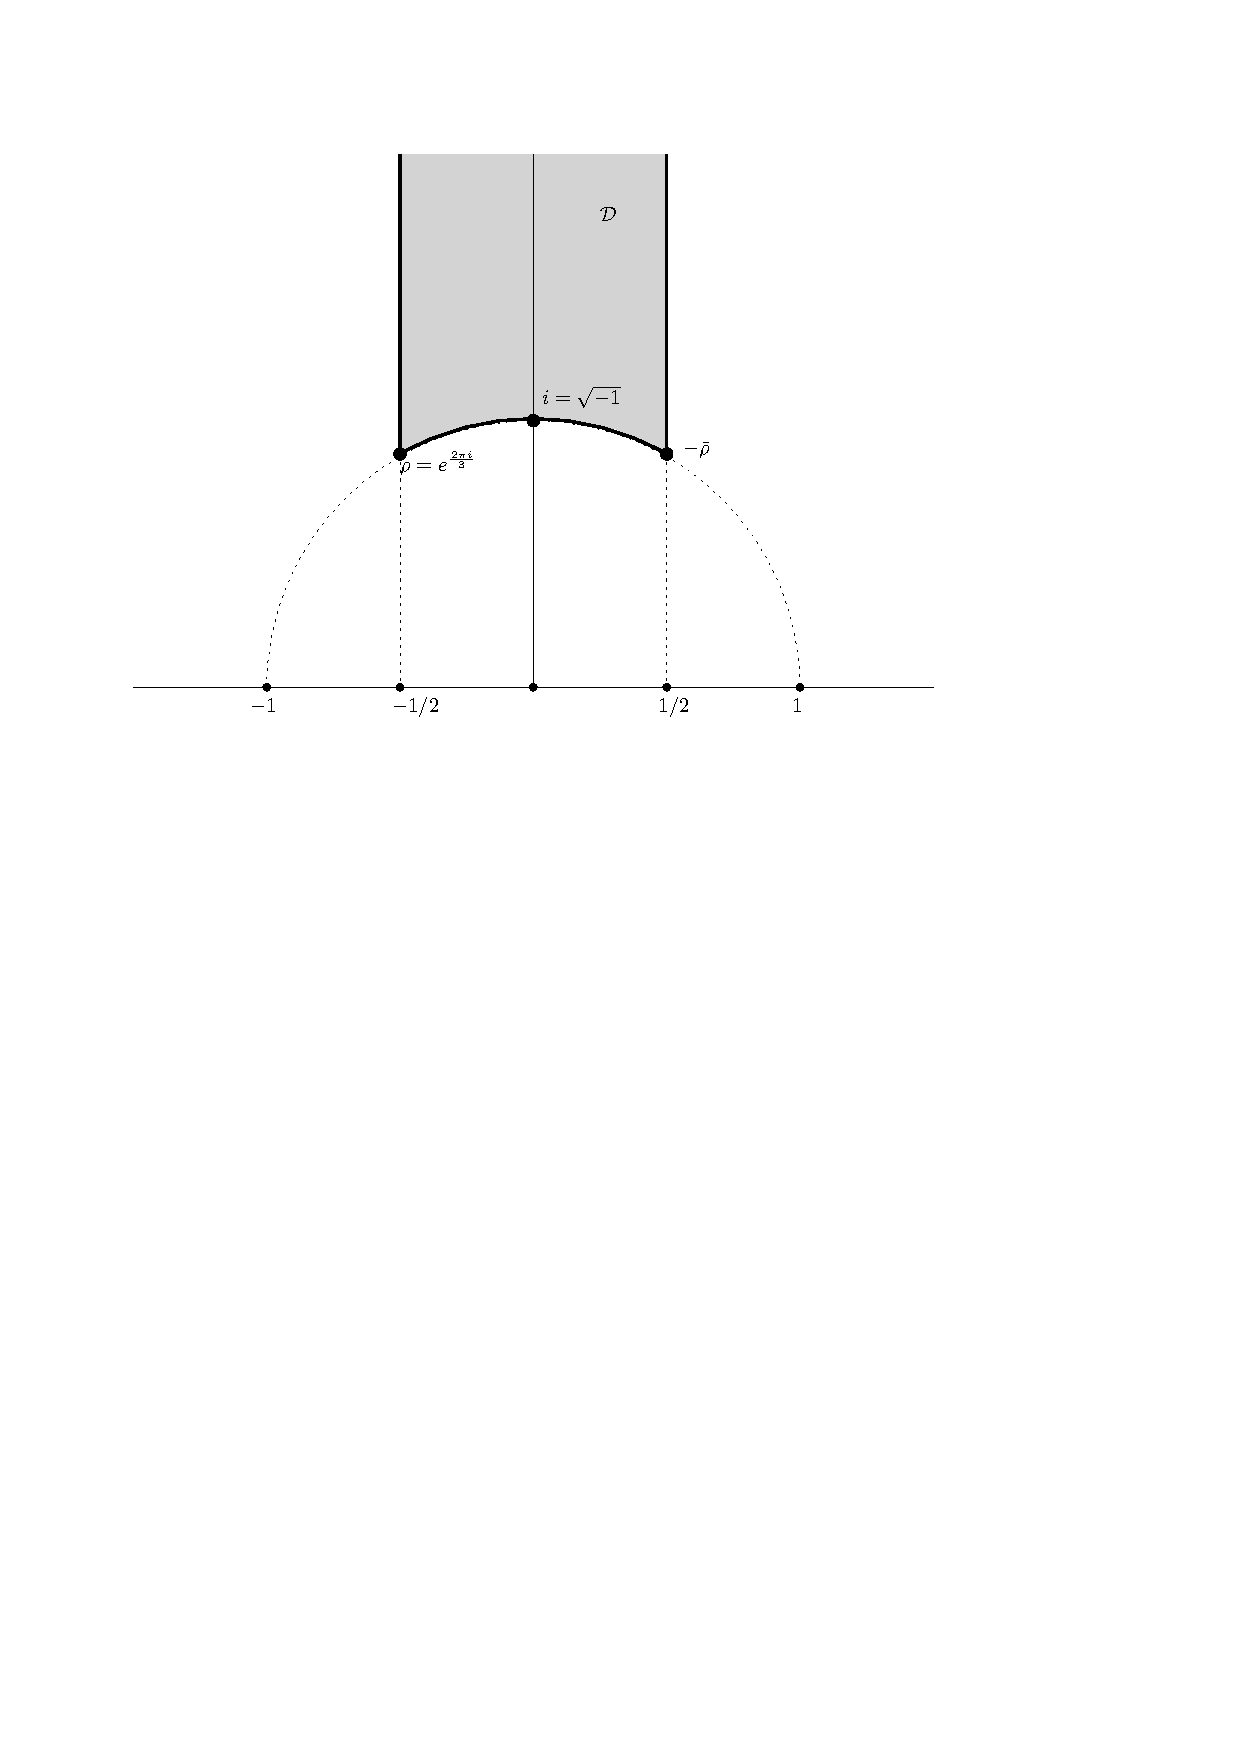
\includegraphics[scale=0.5]{fundomSL2Z.pdf}
\caption{Fundamental domain for $\SL_2(\ZZ)$}
\end{figure}

\begin{definition}
  Let $\Gamma$ be a group acting on $\HH$. A \emphh{fundamental domain} for $\Gamma$ is closed subset $\cD\subset\HH$ such that
  \begin{enumerate}
  \item The set $\cD$ is the closure of its interior.
  \item Every point in $\HH$ is $\Gamma$-equivalent to a point of $\cD$.
  \item If $z,z'\in\cD$ are two distinct points which are $\Gamma$-equivalent then they lie on the boundary of $\cD$.
  \end{enumerate}
\end{definition}

\begin{theorem}
  The subset $\cD$ of $\HH$ as above is a (connected) fundamental domain for $\SL_2(\ZZ)$.

Moreover the stabilizer $H_z$ of a point $z\in\cD$ in $\SL_2(\ZZ)$ is
\[
H_z=\begin{cases}
C_6=\langle ST\rangle = \langle\smtx{0}{-1}{1}{1}\rangle  & z = \rho,\\
C_6'=\langle TS\rangle =\langle \smtx{1}{-1}{1}{0}\rangle & z=\rho + 1,\\
C_4=\langle S\rangle =\langle \smtx{0}{-1}{1}{0}\rangle & z=i,\\
C_2=\langle -I\rangle =\langle \smtx{-1}{0}{0}{-1}\rangle&\text{ else.}
\end{cases}
\]
\end{theorem}
\begin{proof}
  Let $z\in \HH$. We have seen that, if $\gamma\in\SL_2(\ZZ)$, then
\[
\Im(\gamma z) = \frac{\Im(z)}{|cz+d|^2},\quad \gamma = \mtx abcd.
\]
There are finitely many pairs $(c,d)\in\ZZ^2$ such that $|cz+d|<1$. In particular,
one can choose a matrix $\gamma\in\langle S,T\rangle\subseteq \SL_2(\ZZ)$ such that
\[
\Im(\gamma z)\geq \Im(\gamma' z),\quad \forall \gamma'\in \langle S,T\rangle\subseteq\SL_2(\ZZ).
\]
By premultiplying $\gamma$ by an appropriate power of $T$ (which does not change the imaginary part), we may and do assume that $|\Re(\gamma z)|\leq \frac 12$. We will now show that $|\gamma z|\geq 1$:
\[
\Im(\gamma z)\geq \Im(S\gamma z)=\Im(-1/\gamma z)=\frac{\Im(\gamma z)}{|\gamma z|^2}.
\]
This implies $|\gamma z|\geq 1$, and hence $\gamma z\in \cD$, thus proving $(1)$.

In order to show $(2)$, suppose that $z'=\gamma z$ and both $z$ and $z'$ lie in $\cD$. Without loss of
generality, we may assume that $\Im(\gamma z)\geq \Im(z)$, or equivalently that
\[
|cz+d|^2=|cx+d|^2+|cy|^2\leq 1.\quad\text{ (we write $z=x+iy$).}
\]
Since $y>1/2$, this implies that $|c|\leq 1$. The case $c=0$ gives that $|d|\leq 1$ and since $\smtx abcd\in\SL_2(\ZZ)$ this means that $\gamma=\pm\smtx 1 b01$, a translation matrix. Therefore $z'=z\pm 1$.

Let us suppose that $c=1$ (the case $c=-1$ is completely analogous). Then the condition $|z+d|^2\leq 1$ is only satisfied when $|z|=1$ ($d=0$), when $z=\rho$ ($d=1$), or when $z=\rho+1$ ($d=-1$), giving $(2)$.

To study the stabilizers of points $z\in\cD$, we can use the calculations that we have used to show $(2)$. If $\gamma z = z$, then necessarily $c=\pm 1$, and by changing $\gamma$ to $-\gamma$ we may assume $c=1$. The quadratic equation given by $\gamma z = z$ gives that $|a+d|<2$, so $|a+d|\leq 1$. At the same time, the fact that $z\in\cD$ gives $|a-d|\leq 1$. Together, these two inequalities give $|a|\leq 1$. We obtain the following possibilities:
\begin{table}[h]
\begin{tabular}{cccc}
\toprule
$\gamma$&$z$&$z'=\gamma z$&fixed points\\
\midrule
$\pm \smtx 1001$&all&$z$&all\\[5pt]
$\pm \smtx 1101$&$\Re(z)=-\frac 12$&$z+1$&none\\[5pt]
$\pm \smtx 1{-1}01$&$\Re(z)=\frac 12$&$z-1$&none\\[5pt]
$\pm \smtx 0{-1}10$&$|z|=1$&$-1/z$&$i$\\[5pt]
$\pm \smtx {-1}{-1}{1}{0},\pm \smtx{0}{-1}{1}{1}$&$\rho$&$\rho$&$\rho$\\[5pt]
$\pm \smtx {1}{-1}{1}{0},\pm \smtx{0}{-1}{1}{-1}$&$\rho+1$&$\rho+1$&$\rho+1$
\end{tabular}
\end{table}
By studying this table we conclude the classification of stabilizers.
\end{proof}
\begin{corollary}
\label{cor:STgenerate}
  The group $\SL_2(\ZZ)$ is generated by the matrices $T$ and $S$.
\end{corollary}
\begin{proof}
  Let $z_0$ be a point in the interior of $\cD$. Given $\gamma\in\SL_2(\ZZ)$, the theorem provides a matrix $\delta\in\langle T,S\rangle$ such that $\delta\gamma^{-1} z_0\in\cD$. Therefore $\delta\gamma^{-1} z_0 = z_0$ and hence $\delta\gamma^{-1} = \pm I$. Since $S^2=-I$, we are done by possibly multiplying $\delta$ by $S^2$.
\end{proof}

\section{Valence formula}
\label{sec:valence-formula}

Let $f$ be a meromorphic function on some open subset of $\HH$. Write $v_p(f)$ for the order (or valuation) of $f$ at $p\in \HH\cup\{\infty\}$. This is the unique integer
$n$ such that $(z-p)^{-n}f(z)$ is holomorphic and non-vanishing at $p$. If $n$ is positive we
say that $f$ has a zero of order $n$, and if $n$ is negative we say that $f$ has a pole of order $-n$. If $f$ is weakly modular and meromorphic at infinity, then also define $v_\infty(f)=n_0$ if
\[
f(q)=\sum_{n\geq n_0} a_n q^n,\quad a_{n_0}\neq 0.
\]
Next, suppose that $f$ has a Laurent expansion of the form
\[
f(z) = \sum_{n\geq n_0} c_n (z-p)^n.
\]
The \emphh{residue} of $f$ at $p$ is $\res_p(f) = c_{-1}\in\CC$. One can calculate
the order of $f$ at $p$ by using residues, using the following lemma.
\begin{lemma} If $f$ is a meromorphic function around a point $p$, then
  \[
\res_p(f'/f) = v_p(f).
\]
\end{lemma}
\begin{proof}
If $v_p(f)=n$, write $f(z)=(z-p)^ng(z)$ with $g(z)$ holomorphic and non-vanishing at $p$. Then calculate the residue of $f'/f$ by hand.
\end{proof}
We recall without proof two basic results of complex analysis.
\begin{theorem}[Cauchy's integral formula]
  Let $g$ be a holomorphic function on an open subset $U\subseteq\CC$ and let $C$ be a contour in $U$. For each $p\in U$,
\[
\int_C \frac{g(z)}{z-p}dz = 2\pi i g(p).
\]
\end{theorem}
\begin{corollary}
  Let $C(p,r,\alpha)$ be an arc of a circle, of radius $r$ and angle $\alpha$ around a point $p$. If $g$ is holomorphic at $p$, then
\[
\lim_{r\to 0}\int_{C(p,r,\alpha)} \frac{g(z)}{z-p}dz = \alpha i g(p).
\]
\end{corollary}
The following result relates the contour integral of the logarithmic derivative of $f$ to the orders of $f$ at the interior points.
\begin{theorem}[argument principle]
  Let $f$ be a meromorphic function on an open subset $U\subseteq \CC$ and let $C$ be a contour in $U$ not passing through any zeros or poles of $f$. Then:
\[
\int_C\frac{f'(z)}{f(z)}dz = 2\pi i \sum_{z\in\operatorname{int}(C)} v_z(f).
\]
\end{theorem}

\begin{corollary}
  Let $C(p,r,\alpha)$ be an arc of a circle, of radius $r$ and angle $\alpha$ around a point $p$. If $f$ is meromorphic at $p$, then
\[
\lim_{r\to 0}\int_{C(p,r,\alpha)} \frac{f'(z)}{f(z)}dz = \alpha i v_p(f).
\]
\end{corollary}
We will study weakly modular meromorphic functions $f\colon \HH\to \CC$. In this case, the order of vanishing makes sense in $\SL_2(\ZZ)$-orbits: suppose that $f$ has weight $k$. Then an easy computation shows that, for $\gamma\in\SL_2(\ZZ)$,
\[
\lim_{z\to\gamma p} (z-\gamma p)^{-n}f(z) = j(\gamma,p)^{k+2n}\lim_{z\to p} (z-p)^{-n}f(z).
\]
But note now that $j(\gamma,p)$ is nonzero because $p\not\in \QQ\cup\{\infty\}$. We conclude that $v_p(f)=v_{\gamma p}(f)$.

\begin{theorem}[valence formula]
\label{thm:valence-formula}
  Let $f$ be a non-zero weakly modular meromorphic form of weight $k$ on $\SL_2(\ZZ)$. Then:
\[
v_\infty(f)+\frac 12 v_i(f)+\frac 13 v_\rho(f) + \sum_{\tau\in \SL_2(\ZZ)\backslash\HH'} v_\tau(f) = \frac{k}{12}.
\]
Here the sum runs through the orbits in $\SL_2(\ZZ)\backslash\HH$ other than those of $i$ and $\rho$.
\end{theorem}

Before proving this theorem we will see how helpful it is in studying the spaces of modular forms.
\begin{theorem}
  \begin{enumerate}
  \item $M_k=\{0\}$ if $k<0$ or $k = 2$.
  \item $S_k=\{0\}$ if $k < 12$.
  \item $M_0=\CC$.
  \item $S_{12} = \CC\Delta$.
  \end{enumerate}
\end{theorem}
\begin{proof}
  \begin{enumerate}
  \item   Since the left-hand side of the valence formula is non-negative, the right hand side must be non-negative too, hence $k\geq 0$. If $k=2$, then we get $1/6$ on the right-hand side. However, the left-hand side is a sum of non-negative multiples of $1$, $1/2$ and $1/3$, thus a contradiction.
\item   If $0\neq f\in S_k$, then $v_\infty(f)\geq 1$. Therefore the valence formula gives $k\geq 12$.
\item Let $f\in M_0$. Since the constant function $g=f(\infty)$ also belongs to $M_0$, the difference $f-g$ belongs to $S_0=\{0\}$. Therefore $f=g$ is constant, and $M_0=\CC$ is the space of constant functions on $\HH$.
\item  If $f\in S_{12}$, then $v_\infty(f)\geq 1$. Therefore by the valence formula $v_\infty(f)=1$ and $f$ has no other zeros or poles. Define
\[
g(z)=f(z)-\frac{f(i)}{\Delta(i)}\Delta(z).
\]
Then $g(z)\in S_{12}$ and $g(i)=0$. If $g$ is non-zero, then the valence formula applied to $g$ would give a contradiction because $v_\infty(g)\geq 1$ and $v_i(g)\geq 1$. Therefore $g=0$ and $f$ is a multiple of $\Delta$.
  \end{enumerate}
\end{proof}

\begin{corollary}
\begin{enumerate}
  \item For all $k$, we have $S_{k+12} = \Delta M_{k}$.
\item For $k\geq 4$ we have
\[
M_k = (\CC E_k) \oplus S_k
\]
\item 
If $k$ is odd or negative then $M_k = \{0\}$. For each even $k\geq 2$, we have:
\[
\dim(M_k)=\begin{cases}
\lfloor\frac k{12}\rfloor & k\equiv 2\pmod{12},\\
1+ \lfloor\frac k{12}\rfloor & k\not\equiv 2\pmod{12}.
\end{cases}
\]
\end{enumerate}
\end{corollary}

\begin{proof}
For $k<0$ the first statement is trivial, and we just proved it also for  $k=0$. Given $f\in S_{k+12}$, the function $g=f/\Delta$ is holomorphic on $\HH$ because $\Delta$ is non-vanishing, and it belongs to $M_k$ because $v_\infty(g)=v_\infty(f)-v_\infty(\Delta)=v_\infty(f)-1\geq 0$.

Consider the linear map
\[
\varphi\colon M_k\to\CC,\quad f\mapsto f(\infty).
\]
Then $S_k=\ker\varphi$. Also $\varphi$ is surjective because $\varphi(E_k)=1$. Therefore $M_k=\CC E_k\oplus S_k$.

Note that this gives a recursive way to obtain $M_k$:
\[
M_k = \CC E_k \oplus S_k = \CC E_k \oplus (\Delta M_{k-12}).
\]

For $k$ odd we know that $M_k=\{0\}$ by the weak-modularity condition. For $k<0$ we also know $M_k=\{0\}$ by the previous part. We prove the remaining formula by induction on $k$. Note that we already know it for $k=0$ and $k=2$. For $k=4, 6, 8, 10$ then since $\dim(M_k)=1+\dim(S_k)=1+\dim(M_{k-12}) = 1$ we get $\dim(M_k)=1$. If $k$ is even and $k\geq 12$, then:
\[
\dim(M_k)=1+\dim(M_{k-12}).
\]
\end{proof}
\begin{corollary}
  The space $M_k$ has for basis the following set:
\[
M_k=\langle E_4^aE_6^b~|~ a\geq 0,b\geq 0, 4a+6b=k\rangle.
\]
\end{corollary}
\begin{proof}
  We start by showing that the given monomials $E_4^aE_6^b$ generate $M_k$. For $k=2,4,6$ this is clear because we know $M_2=\{0\}$, and $M_4=\CC E_4$ and $M_6=\CC E_6$. For $k\geq 8$ we induct on $k$. Choose some
 pair $(a,b)$ such that $4a+6b=k$ (convince yourself that this is always possible). If $f\in M_k$, then since $E_4^aE_6^b (\infty)=1$, the function $g(z)=f(z)-f(\infty)E_4^aE_6^b$ is a cusp form in $S_k$. Therefore $g=\Delta h$, for
some $h\in M_{k-12}$. By induction hypothesis, $h$ is a linear combination of monomials $E_4^xE_6^y$ for appropriate pairs $(x,y)$. Using the expression $\Delta=\frac{1}{1728}(E_4^3-E_6^2)$ we deduce the result for $f$.

Now we show that the given monomials are linearly independent. We can use induction on $k$ in steps of $12$ once more, to show that the number of such monomials agrees with $\dim M_k$. This can be checked by hand for $k\leq 14$. Suppose that $k\geq 14$. Note that each monomial $E_4^aE_6^b$ of weight $k-12$ gives a monomial $E_4^aE_6^{b+2}$ of weight $k$. All such monomials are obtained in this way, except for those of the form $E_4^a$ or $E_4^aE_6$. When $k\equiv 0\pmod 4$ then $E_4^{k/4}$ is of weight $k$, and when $k\equiv 2\pmod 4$ then $E_4^{(k-6)/2}E_6$ is of weight $k$, thus in any case there is exactly one more monomial of weight $k$ than there are of weight $k-12$. This completes the proof.
\end{proof}

\begin{example}
  This allows to write down all spaces of modular and cusp forms for $\SL_2(\ZZ)$. For example,
\[
M_{18} = \CC E_{18}\oplus S_{18} = \CC E_{18} \oplus \Delta M_6 = \CC E_{18}\oplus \CC\Delta E_6.
\]
\[
M_{30} = \CC E_{30} \oplus \CC\Delta E_{18} \oplus \CC \Delta^2 E_6.
\]
Another basis for the same space (which is better because it is expressed in terms of $E_4$, $E_6$ and $\Delta$):
\[
M_{30} = \CC E_6^5\oplus \Delta E_6^3 \oplus \Delta^2 E_6.
\]
Note that these forms are linearly independent (why?). Since $\dim M_{30}=3$, they form a basis.
\end{example}

\begin{remark}
  Suppose that $f(z)$ is a non-zero weakly-modular form of weight $0$. Then $f(\gamma z)=f(z)$. By the valence formula, $f$ has the same number of zeros as poles. This number is called the \emphh{valence} of $f$, and hence the name for the theorem.
\end{remark}

Another very powerful application of the valence formula is the following:
\begin{theorem}
  Let $f$ be a modular form of weight $k$. Suppose that $f$ has a $q$-expansion of the form $\sum_{n\geq 0} a_nq^n$. If $a_j=0$ for all $0\leq j\leq k/12$, then $f=0$.
\end{theorem}
\begin{proof}
  The hypothesis means that $v_\infty(f) > k/12$. This is incompatible with the valence formula, and thus $f$ must be zero.
\end{proof}
\begin{corollary}
  Let $f$ and $g$ be two modular forms of the same weight $k$, and suppose that their $q$-expansions coincide for the first $\lfloor k/12\rfloor$ coefficients. Then $f=g$.
\end{corollary}

\subsection{The modular invariant \texorpdfstring{$j$}{j}}
  Define the function
\[
j(z)=\frac{E_4^3}{\Delta} = \frac{1+\cdots}{q+\cdots} = q^{-1} + 744 + 196884 q + \cdots.
\]
\begin{proposition}
  \begin{enumerate}
  \item $j$ is a meromorphic weakly-modular form of weight $0$.
  \item $j$ is holomorphic on $\HH$ and has a simple pole at infinity.
  \item It induces a bijection $\SL_2(\ZZ)\backslash\HH\to \CC$.
  \end{enumerate}
\end{proposition}
\begin{proof}
The fact that $j$ it is meromorphic weakly-modular of weight $0$ follows from it being a quotient of two modular forms of weight $12$.

Since $E_4$ is non-vanishing at infinity and $\Delta$ has a simple zero then $j=E_4^3/\Delta$ has a simple pole at infinity (we can also see it from its $q$-expansion, which starts with $q^{-1}$). The valence formula shows that $v_\rho(E_4)=1$, and therefore $j(z)$ has a triple zero at $\rho$. It is holomorphic on $\HH$ because $\Delta$ is non-vanishing on $\HH$.

Fix $c\in\CC$. The function $j(z)-c=q^{-1}+744-c+\cdots$ is another meromorphic weakly-modular function of weight $0$ and has a simple pole at $\infty$. The valence formula gives in this case that $j(z)-c$ has exactly one zero on $\SL_2(\ZZ)\backslash\HH$. This gives the last claim.
\end{proof}

\subsection{Proof of the valence formula}
The proof presented here avoids algebraic geometry, at the cost of some complex analysis. Let
$f$ be a modular function, and consider the following contour:
\begin{figure}[h]
  \centering
  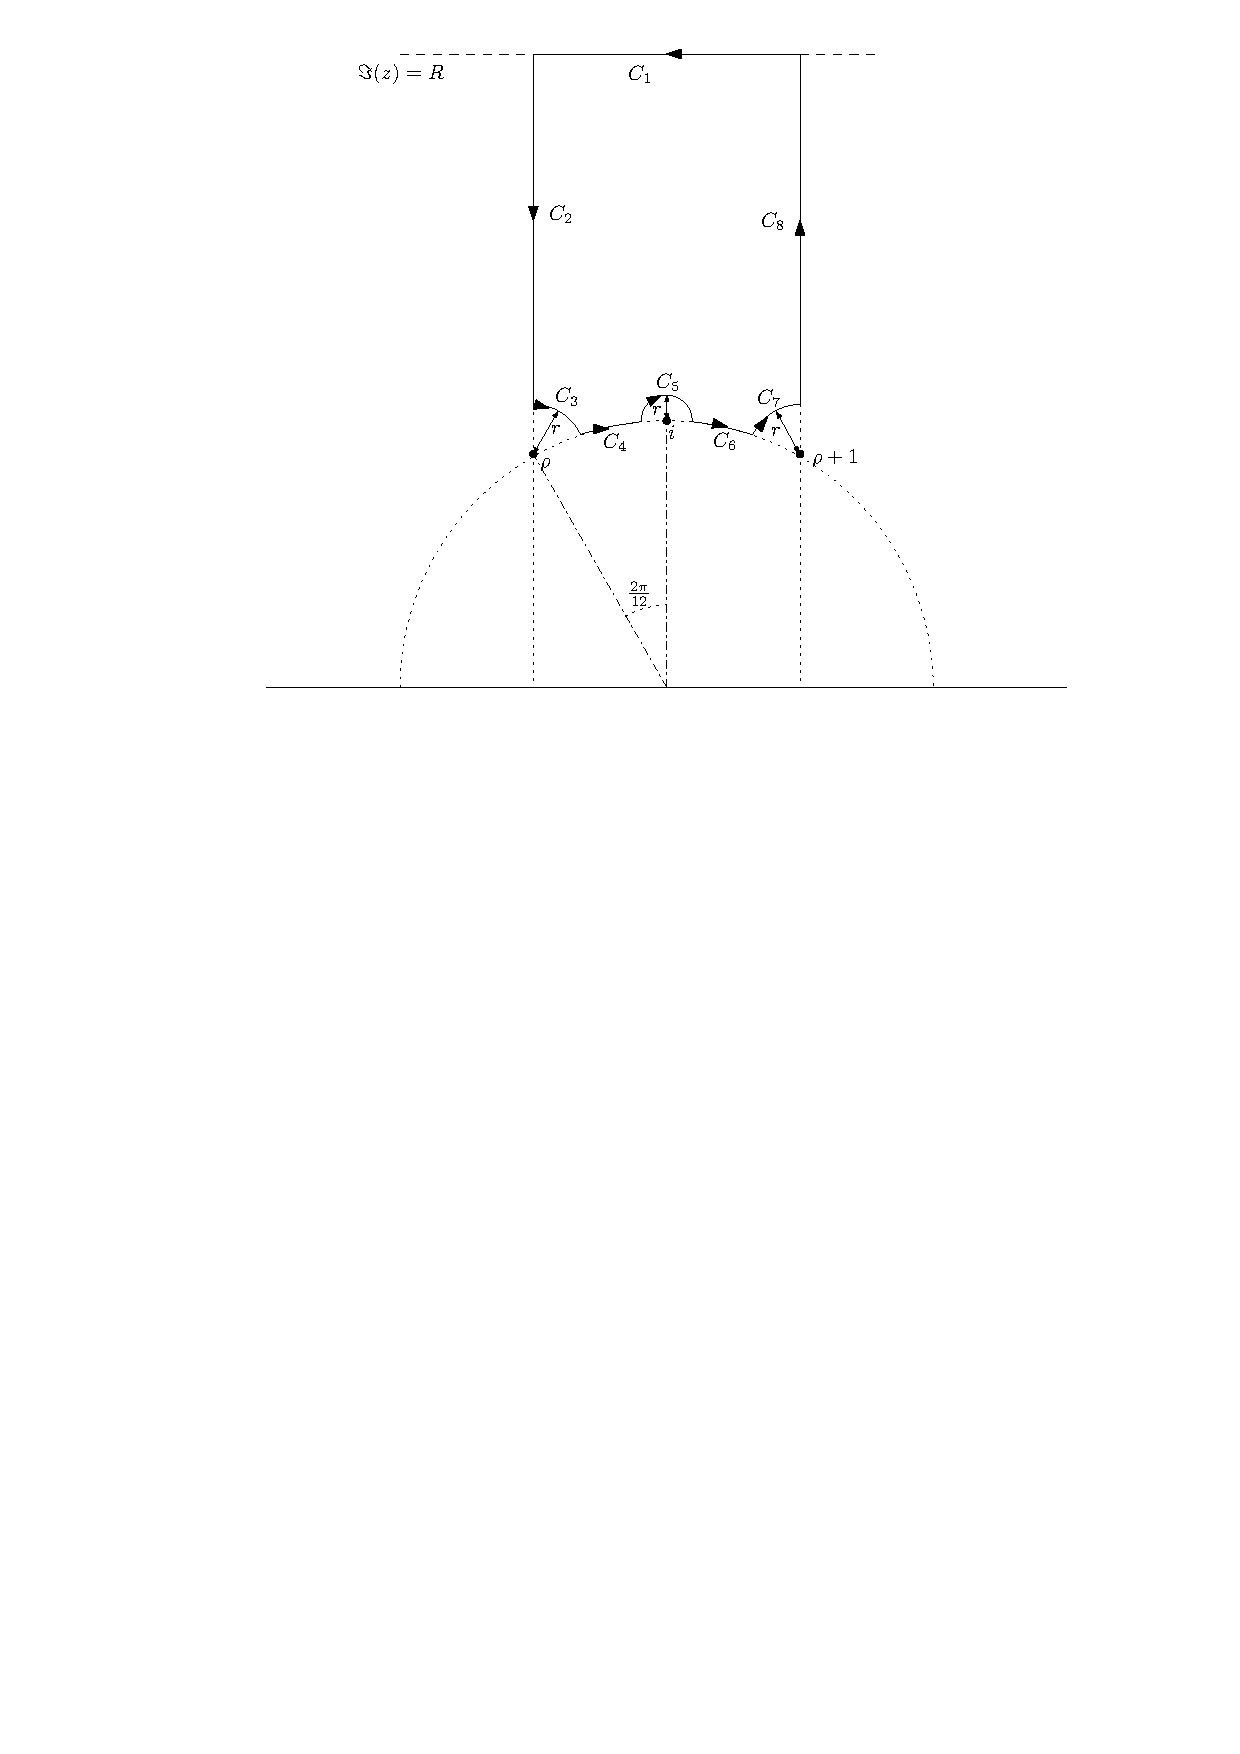
\includegraphics[height=6cm]{contour.pdf}
  \caption{Contour to integrate}
  \label{fig:contour}
\end{figure}

The proof consists in integrating $f'(z)/f(z)$ around the indicated contour $C$ in two different ways.
\paragraph{Integral residue formula:} This is the first way in which we calculate the contour integral. For $R$ large enough so that the contour contains all zeros and poles of $\SL_2(\ZZ)\backslash\HH'$ with large imaginary part, we have:
\[
\int_C \frac{f'(z)}{f(z)}dz = 2\pi i \sum_{p\in\operatorname{int}(C)} \res_p\left(\frac{f'}{f}\right) = 2\pi i\sum_{p\in \SL_2(\ZZ)\backslash\HH'} v_p(f).
\]
The rest of the proof consists in computing the integral as the sum of the path integrals along $C_1$,\ldots, $C_8$.
\paragraph{Integral along $C_1$:} Perform the change of variables $q(z)=e^{2\pi i z}$. Note that:
\[
dq = 2\pi i qdz,\quad dz = \frac{1}{2\pi i}\frac{dq}{q}.
\]
Moreover, the path $q(C_1)$ is a clockwise circle of radius $e^{-2\pi R}$ centered around $0$. Finally,
\[
\frac{d}{dz}f(q) = \frac{d}{dz} f(e^{2\pi i z}) = 2\pi i q f'(q).
\]
Putting these together, we obtain:
\[
\int_{C_1}\frac{f'(z)}{f(z)}dz = \int_{q(C_1)} \frac{f'(q)}{f(q)} dq.
\]
Since $f$ is meromorphic around infinity, this last quantity equals $- v_\infty(f)$.

\paragraph{Integral along $C_2$ and $C_8$:} Note that since $f$ is modular it satisfies $f(z+1)=f(z)$. Therefore also $f'(z+1)=f'(z)$, and we get, by changing $w=z+1$:
\begin{align*}
\int_{C_8}\frac{f'(w)}{f(w)}dw &= -\int_{C_2}\frac{f'(z+1)}{f(z+1)}dz = -\int_{C_2}\frac{f'(z)}{f(z)}dz.
\end{align*}
Therefore the contributions of $C_2$ and $C_8$ cancel out.

\paragraph{Integral along $C_4$ and $C_6$:} In the same way that for $C_2$ and $C_8$ we considered the change $z\mapsto z+1$, here we consider the change $z\mapsto s(z)=-z^{-1}$. This change of variables transforms $C_4$ to $-C_6$. Weak-modularity of $f$ implies also that $f(z) = z^{-k}f(s(z))$. Differentiating both sides yields:
\[
f'(z) = -kz^{-k-1}f(s(z)) + z^{-k}f'(s(z))s'(z).%\implies z^{-k}f'(-z^{-1})z^{-2} = -f'(z) - kz^{-k-1}f(-z^{-1}).
\]
This gives
\[
\frac{f'(z)}{f(z)} = \frac{-k}{z} + \frac{f'(s(z))s'(z)}{f(s(z))}.
\]
Therefore we may compute
\begin{align*}
\int_{C_4}\frac{f'(z)}{f(z)}dz &=\int_{C_4} \frac{-k}{z}dz + \int_{C_4}\frac{f'(s(z))s'(z)}{f(s(z))}dz =2\pi i\frac{k}{12} +\int_{-C_6}\frac{f'(s)}{f(s)}ds,
\end{align*}
and hence
\[
\int_{C_4+C_6}\frac{f'(z)}{f(z)}dz \to_{r\to 0} 2\pi i\frac{k}{12}.
\]

\paragraph{Integral along $C_5$:} Using the argument principle we obtain
\[
\int_{C_5} \frac{f'(z)}{f(z)}dz \stackrel[r\to 0]{}\longrightarrow -\frac 12 2\pi i v_i(f).
\]

\paragraph{Integrals along $C_3$ and $C_7$:} Applying again the argument principle we obtain
\[
\int_{C_3} \frac{f'(z)}{f(z)}dz \stackrel[r\to 0]{}\longrightarrow -\frac 16 2\pi i v_\rho(f),\text{ and}\quad
\int_{C_5} \frac{f'(z)}{f(z)}dz \stackrel[r\to 0]{}\longrightarrow -\frac 16 2\pi i v_{\rho+1}(f)=-\frac{1}{6}2\pi i v_\rho(f).
\]
Therefore
\[
\int_{C_3+C_5} \frac{f'(z)}{f(z)}dz \stackrel[r\to 0]{}\longrightarrow -\frac{1}{3}2\pi i v_\rho(f).
\]

\paragraph{Conclusion:} Putting together all the above calculations yields the sought formula.\qed

\section{A product formula for \texorpdfstring{$\Delta(z)$}{Delta(z)}}
\label{sec:a-product-formula-for-Delta}

Consider the weight-$2$ Eisenstein series
\[
G_2(z)=\sum_c\sumprime_d \frac{1}{(cz+d)^2},
\]
which does not converge absolutely. It is \emph{not} a weight-$2$ modular form (there are no such other than $0$), but we still have the formula:
\[
G_2(z)=2\zeta(2)E_2(z),\quad E_2(z)=1-24\sum_{n=1}^\infty \sigma_1(n)q^n.
\]
The function $E_2(z)$ is holomorphic on $\HH$, and $E_2(z+1)=E_2(z)$. However, we are about to see that
\[
z^{-2}E_2(-1/z) = E_2(z)+\frac{12}{2\pi i z}.
\]
Sometimes these functions are called \emphh{quasi-modular}.

\begin{theorem}
The function  $G_2$ satisfies $G_2(z+1)=G_2(z)$ and  it has the $q$-expansion
\[
G_2(z) = 2\zeta(2) - 8\pi^2\sum_{n=1}^\infty \sigma_1(n)q^n,\quad q=e^{2\pi i z}.
\]
Moreover, $G_2$ satisfies the transformation property:
\begin{equation}
\label{eq:G2}
G_2(\gamma z) = (cz+d)^2G_2(z)- 2\pi i c(cz+d),\quad \gamma=\mtx abcd.
\end{equation}
In particular, the non-holomorphic function  $G_2^*(z) = G_2(z)-\pi/\Im(z)$ is weight-$2$-invariant for $\SL_2(\ZZ)$.
\end{theorem}
\begin{proof}

To show that $G_2(z+1)=G_2(z)$, we must show that
\[
\sum_{n\neq 0}\frac{1}{(m(z+1)+n)^2} = \sum_{n\neq 0} \frac{1}{(mz+n)^2}.
\]
This follows from the fact that the sum converges absolutely and $n\mapsto n+m$ is a bijection of $\ZZ$ (for each fixed $m\in\ZZ$).

Next, we compute the $q$-expansion of $G_2$. First, note that
\[
G_2(z)=2\zeta(2)+2\sum_{m=1}^\infty \sum_{n\in\ZZ}\frac{1}{(mz+n)^2}.
\]
Using now Lemma~\ref{lemma:expansion-latticesum} with $z$ substituted by $mz$, we obtain
\[
G_2(z)=2\zeta(2)-8\pi^2\sum_{m=1}^\infty\sum_{d=1}^\infty dq^{md}.
\]
Grouping terms contributing to a given power of $q$ gives the formula.

Next, by expanding $G_2(\gamma_1\gamma_2z)$, using the cocycle property of $j(\gamma,z)$ and calculating the lower left entry of the product of two matrices, we see that if Equation~\ref{eq:G2} is satisfied for matrices $\gamma_1$ and $\gamma_2$ then it is also satisfied for $\gamma_1\gamma_2$ and $\gamma_1^{-1}$. Therefore to prove Equation~\ref{eq:G2} it will be enough to prove it for the matrix $S=\smtx{0}{-1}{1}{0}$.

We next show that
\[
G_2(-1/z) = z^2 \left(2\zeta(2) + \sum_{n\in\ZZ}\sum_{m\neq 0}\frac{1}{(mz+n)^2}\right).
\]
This only differs from $z^2G_2(z)$ in the order of summation! This is done by substituting $-1/z$ in the definition to get:
\[
G_2(-1/z) = \sum_{n\neq 0} \frac 1{n^2} + \sum_{m\neq 0}\sum_{n\in\ZZ}\frac{z^2}{(mz-n)^2} = \sum_{n\neq 0} \frac 1{n^2} + \sum_{m\neq 0}\sum_{n\in\ZZ}\frac{z^2}{(m-nz)^2}
\]
This can be rewritten as
\[
2\zeta(2) + z^2\left(\sum_{n\neq 0}\sum_{m\neq 0}\frac{1}{(mz+n)^2}\right)=2\zeta(2)+z^2\left(\sum_{n\neq 0}\sum_{m\neq 0} \frac{1}{(mz+n)^2} + 2\zeta(2)\right).
\]
The outer term $2\zeta(2)$ can be put into the sum corresponding to the term $n=0$, getting the desired formula. The partial fraction decomposition
\[
\frac{1}{(mz+n)(mz+n+1)} = \frac{1}{mz+n}-\frac{1}{mz+n+1}
\]
allows us to show (via a telescoping sum) that
\[
\sum_{m\neq 0} \sum_{n\in\ZZ} \frac{1}{(mz+n)(mz+n+1)} = 0
\]
Subtracting this series from the definition of $G_2(z)$ (which can be done term by term, this only needs conditional convergence) we get the new formula involving an absolutely convergent sum:
\[
G_2(z)=2\zeta(2)+\sum_{\substack{m\neq 0\\n\in\ZZ}} \frac{1}{(mz+n)^2(mz+n+1)}.
\]

Then we compute
\[
z^{-2}G_2(-1/z)-G_2(z) = \sum_{n\in\ZZ}\sum_{m\neq 0}\frac{1}{(mz+n)^2} - \sum_{m\neq 0,n\in\ZZ} \frac{1}{(mz+n)^2(mz+n+1)}.
\]
Subtracting term by term and using that
\[
\frac{1}{(mz+n)^2} - \frac{1}{(mz+n)^2(mz+n+1)} = \frac{1}{(mz+n)(mz+n+1)}
\]
gives an alternative formula for $G_2(z)$:
\[
G_2(z) = z^{-2}G_2(-1/z) - \sum_{n\in\ZZ}\sum_{m\neq 0} \frac{1}{(mz+n)(mz+n+1)}.
\]

Finally, consider the sum
\[
\lim_{N\to\infty} \sum_{n=-N}^{N-1}\sum_{m\neq 0}\left(\frac{1}{mz+n}-\frac{1}{mz+n+1}\right).
\]
For each fixed $N$ we can reverse the sum and calculate, since the inner sum telescopes:
\begin{align*}
\sum_{m\neq 0}\sum_{n=-N}^{N-1} \left(\frac{1}{mz+n}-\frac{1}{mz+n+1}\right) &= \sum_{m\neq 0} \left(\frac{1}{mz-N} - \frac{1}{mz+N}\right)\\
&=\frac{-1}{z}\sum_{m\neq 0}\left( \frac{1}{N/z + m}+\frac{1}{N/z-m}\right)\\
&=\frac{-2\pi}{z}\cot(\pi N/z).
\end{align*}
Taking the sum as $N\to \infty$ and using that
\[
\pi\cot(\pi N/z)=\pi i-2\pi i\sum_{m=0}^\infty e^{2\pi i mN/z}
\]
we get the formula:
\[
\lim_{N\to\infty} \sum_{n=-N}^{N-1}\sum_{m\neq 0}\left(\frac{1}{mz+n}-\frac{1}{mz+n+1}\right)=-\frac{2\pi i}{z}.
\]
This finishes the proof.
\end{proof}

\subsection{The Dedekind-eta function}
\label{sec:dedekind-eta}

Define $\eta(z)$ as through the following product
\[
\eta(z) = q^{1/24}\prod_{n=1}^\infty (1-q^n).
\]
The function $\eta(z)$ is holomorphic and non-vanishing on $\HH$ (to check it, it is enough to check that $\sum q^n$ converges absolutely and uniformly on compact subsets of $\HH$).
\begin{theorem}
The $\eta$ function satisfies the following transformation property:
  \[
\eta(-1/z) = \sqrt{z/i} \eta(z).
\]
\end{theorem}
\begin{proof}
  Note that:
\begin{align*}
\frac d{dz} \log\eta(z) &= \frac{2\pi i}{24}  + \sum_{n=1}^\infty\frac{-2\pi i n q^n}{1-q^n} =\frac{2\pi i}{24}\left(1-24\sum_{n=1}^\infty \frac{nq^n}{1-q^n}\right)\\
&=\frac{\pi i}{12}\left(1-24\sum_{n=1}^\infty n\sum_{m=1}^\infty q^{nm}\right)=\frac{\pi i}{12} E_2(z).
\end{align*}
Using quasi-modularity of $E_2$, we deduce:
\[
\dlog \left(\eta(-1/z)\right) = \dlog \left(\sqrt{z/i} \eta(z)\right).
\]
Therefore $\eta(-1/z) = C \sqrt{z/i} \eta(z)$ and setting $z=i$ one gets $C=1$, as we wanted.
\end{proof}


\begin{theorem}
  \[
\Delta = q\prod_{n=1}^\infty (1-q^n)^{24}.
\]
\end{theorem}
\begin{proof}
  Note that:\[
\eta^{24}(z)=q\prod_{n=1}^\infty (1-q^n)^{24},
\]
so $\eta^{24}(z+1)=\eta^{24}(z)$. Moreover,
\[
\eta^{24}(-1/z) = z^{12}\eta^{24}(z).
\]
Since $\eta^{24}(z)=q+\cdots$ and $\eta^{24}(z)\in S_{12} = \CC\Delta$, we deduce that $\eta^{24}=\Delta$.
\end{proof}

\section{Growth of Fourier coefficients}
In this final section we study the different behavior of the Fourier coefficients of a modular form $f$, depending on whether $f$ is cuspidal or not. Intuitively, if $f$ is cuspidal, the vanishing at infinity should force the coefficients to grow slower.

We start by studying Eisenstein series.
\begin{proposition}
\label{prop:growtheistenstein}
  The Fourier coefficients $a_n(E_k)$ of the Eisenstein series $E_k$ grow as $n^{k-1}$. Precisely, there exist constant $A,B>0$ such that
\[
An^{k-1}\leq |a_n(E_k)|\leq B n^{k-1}.
\]
\end{proposition}
\begin{proof}
  We will use that the Fourier coefficients of $E_k$ have a simple formula:
\[
E_k = 1+C_k\sum_{n=1}^\infty \sigma_{k-1}(n)q^n,
\]
and hence $|a_n(E_k)|=|C_k|\sigma_{k-1}(n)$.
Therefore
\[
|a_n(E_k)|=|C_k|\sum_{d\mid n} d^{k-1} \geq |C_k|n^{k-1},
\]
and we may take $A=|C_k|$. On the other hand,
\[
\frac{|a_n(E_k)|}{n^{k-1}} = |C_k|\sum_{d\mid n} \left(\frac{d}{n}\right)^{k-1} = |C_k|\sum_{d\mid n} \frac{1}{d^{k-1}}.
\]
This last term can be coarsely estimated:
\[
|C_k|\sum_{d\mid n} \frac{1}{d^{k-1}}\geq |C_k|\sum_{d=1}^\infty \frac{1}{d^{k-1}} = |C_k|\zeta(k-1).
\]
Hence we may take $B=|C_k|\zeta(k-1)$.
\end{proof}

The following result shows that the coefficients of cusp forms grow much slower.
\begin{theorem}[Hecke]
\label{theorem:growthcusps}
  If $\sum_{n=1}^\infty a_nq^n$ is the $q$-expansion of a  cusp form of weight $k$, then $a_n=O(n^{k/2})$. Precisely, there is a constant $M>0$ such that
\[
|a_n|\leq Mn^{k/2}.
\]
\end{theorem}
\begin{proof}
  Note that as $q\to \infty$ we have $|f(z)|=O(q)=O(e^{-2\pi i})$, where $y=\Im(z)$.  Consider the function
\[
\phi(z)=|f(z)|y^{k/2}.
\]
It is a continuous function $\HH\to \RR_{\geq 0}$, and it is invariant under $\SL_2(\ZZ)$. Since $\phi$ approaches $0$ as $y$ approaches infinity, we deduce that $\phi$ is bounded: $|f(z)|\leq M' y^{-k/2}$ for all $z\in\HH$. Since $f(z)q^{-n-1} = \cdots +a_nq^{-1} + a_{n+1} + a_{n+2} q + \cdots$ the residue theorem implies that
\[
a_n = \frac{1}{2\pi i} \int_{C_y} f(z)q^{-n-1}dq,
\]
where $C_y$ is the counter-clockwise circle described by $e^{2\pi i (x+iy)}$ when $y$ is fixed and $x$ moves from $0$ to $1$. This gives:
\[
a_n=\int_0^1 f(x+iy)q^{-n}dx,
\]
Using the bound for $|f|$ we obtain:
\[
|a_n|\leq \int_0^1 M' y^{-k/2}|e^{-2\pi i n (x+iy)}dx = M'y^{-k/2} e^{2\pi yn}.
\]
This expression is valid for all $y>0$. In particular, for $y=1/n$ we get $|a_n|\leq M'e^{2\pi} n^{k/2}$. Setting $M=M'e^{2\pi}$ finishes the proof.
\end{proof}
\begin{corollary}
\label{corollary:growthmodforms}
  If $f$ is not a cusp form, then the coefficients $a_n$ grow as $n^{k-1}$.
\end{corollary}
\begin{proof}
If $f$ is a modular form of weight $k$, write $f=\lambda E_k + h$, where $h$ is a cusp form. The hypothesis of $f$ not being a cups form translates in $\lambda\neq 0$. Therefore
\[
a_n(f)=\lambda a_n(E_k)+a_n(h).
\]
Since $n^{k-1}$ grows much faster than $n^{k/2}$ and $\lambda\neq 0$, we deduce that $a_n(f)$ grows as $n^{k-1}$.
\end{proof}


%%% Local Variables: 
%%% mode: latex
%%% TeX-master: "main"
%%% End: 
